\chapter{다중 컨테이너 환경}
지난 섹션에서는 Docker로 응용 프로그램을 실행하는 것이 얼마나 쉽고 재미있는지 살펴보았습니다. 간단한 정적 웹사이트로 시작하여 Flask 앱을 시도했습니다. 둘 다 몇 번의 명령만으로 로컬과 클라우드에서 실행할 수 있었습니다. 이 두 응용 프로그램의 공통점은 단일 컨테이너에서 실행된다는 것입니다.

프로덕션에서 서비스를 실행한 경험이 있는 분들은 요즘의 응용 프로그램이 그렇게 단순하지 않다는 것을 알고 있을 것입니다. 거의 항상 데이터베이스(또는 다른 종류의 영구 저장소)가 관련되어 있습니다. Redis 및 Memcached와 같은 시스템은 대부분의 웹 응용 프로그램 아키텍처에서 필수적인 요소가 되었습니다. 따라서 이 섹션에서는 다른 서비스를 필요로 하는 응용 프로그램을 Dockerize하는 방법을 배우는 데 시간을 할애할 것입니다.

특히, 다중 컨테이너 Docker 환경을 실행하고 관리하는 방법을 살펴보겠습니다. 왜 다중 컨테이너일까요? Docker의 주요 포인트 중 하나는 제공하는 격리 방식입니다. 프로세스와 종속성을 샌드박스(컨테이너라고 함)로 묶는 아이디어가 매우 강력합니다.

응용 프로그램 계층을 분리하는 것이 좋은 전략인 것처럼 각 서비스를 위한 컨테이너를 분리하는 것이 현명합니다. 각 계층은 서로 다른 리소스 요구 사항을 가질 가능성이 높으며 이러한 요구 사항은 다른 속도로 증가할 수 있습니다. 각 계층을 다른 컨테이너로 분리하면 서로 다른 리소스 요구 사항에 따라 가장 적절한 인스턴스 유형을 사용할 수 있습니다. 이는 전체 마이크로서비스 운동과도 잘 맞습니다. 이는 Docker(또는 다른 컨테이너 기술)가 현대 마이크로서비스 아키텍처의 선두에 서 있는 이유 중 하나입니다.

\section{SF 푸드 트럭}
Dockerize할 앱은 SF 푸드 트럭입니다. 이 앱을 만들 때 목표는 유용한(실제 세계의 응용 프로그램을 닮은) 것이며, 최소한 하나의 서비스에 의존하지만 이 튜토리얼의 목적에는 너무 복잡하지 않은 것을 만드는 것이었습니다. 이것이 제가 생각해낸 것입니다.

\begin{figure}
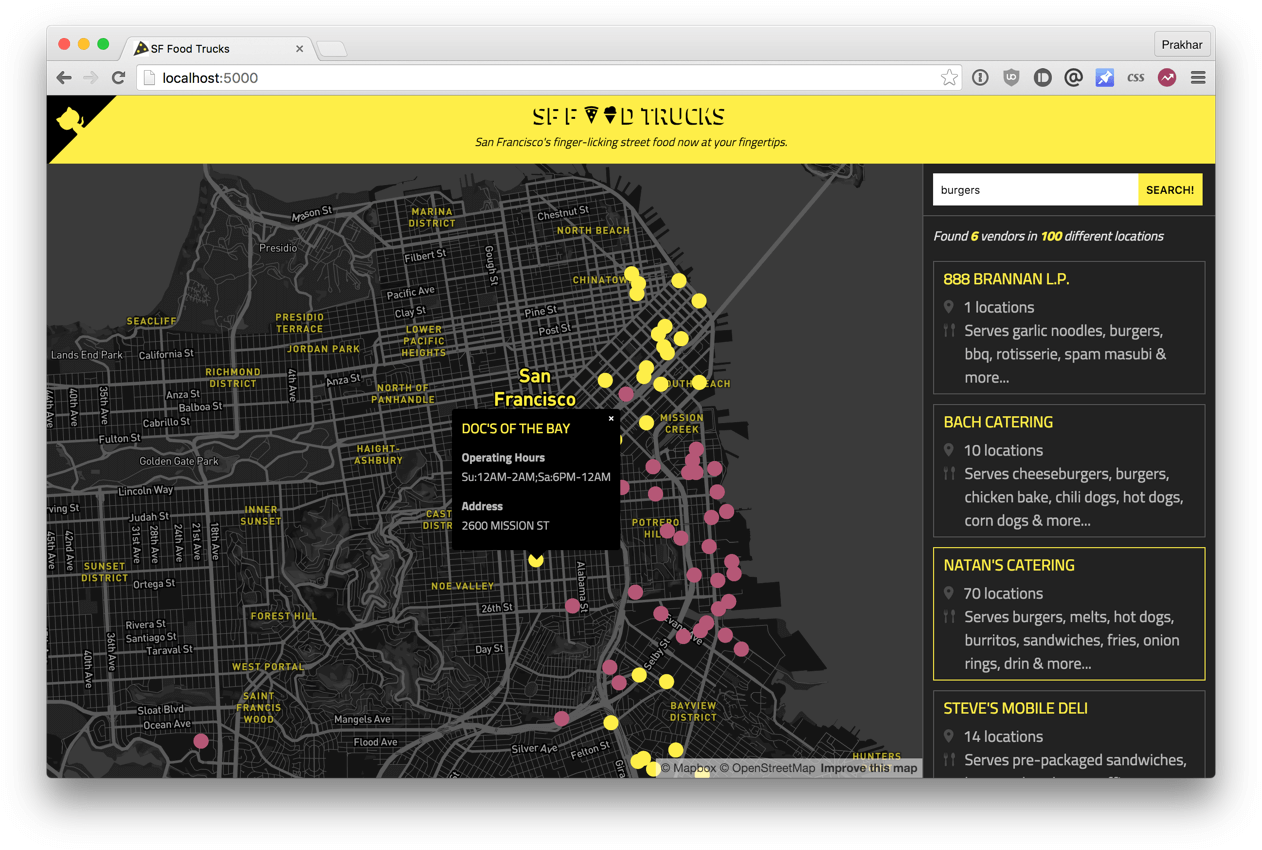
\includegraphics[width=\textwidth]{images/foodtrucks.png}
\caption{SF Food Trucks}
\end{figure}

이 앱의 백엔드는 Python(Flask)으로 작성되었으며 검색에는 Elasticsearch를 사용합니다. 이 튜토리얼의 다른 모든 것처럼 전체 소스 코드는 Github에서 사용할 수 있습니다. 이 앱을 다중 컨테이너 환경으로 구축, 실행 및 배포하는 방법을 배우기 위한 후보 응용 프로그램으로 사용할 것입니다.

먼저 로컬 저장소를 클론해 봅시다.
\begin{verbatim}
$ git clone https://github.com/prakhar1989/FoodTrucks
$ cd FoodTrucks
$ tree -L 2
.
├── Dockerfile
├── README.md
├── aws-compose.yml
├── docker-compose.yml
├── flask-app
│   ├── app.py
│   ├── package-lock.json
│   ├── package.json
│   ├── requirements.txt
│   ├── static
│   ├── templates
│   └── webpack.config.js
├── setup-aws-ecs.sh
├── setup-docker.sh
├── shot.png
└── utils
    ├── generate_geojson.py
    └── trucks.geojson
\end{verbatim}

flask-app 폴더에는 Python 응용 프로그램이 있으며, utils 폴더에는 데이터를 Elasticsearch에 로드하는 유틸리티가 있습니다. 디렉토리에는 일부 YAML 파일과 Dockerfile도 포함되어 있으며, 이 튜토리얼을 진행하면서 자세히 살펴볼 것입니다. 궁금하다면 파일을 살펴보세요.

이제 흥미가 생겼다면(희망적으로) 앱을 Dockerize하는 방법을 생각해 봅시다. 응용 프로그램은 Flask 백엔드 서버와 Elasticsearch 서비스로 구성되어 있습니다. 이 앱을 분할하는 자연스러운 방법은 Flask 프로세스를 실행하는 컨테이너와 Elasticsearch(ES) 프로세스를 실행하는 컨테이너로 나누는 것입니다. 이렇게 하면 앱이 인기를 얻으면 병목 현상이 발생하는 곳에 따라 더 많은 컨테이너를 추가하여 확장할 수 있습니다.

좋습니다, 우리는 두 개의 컨테이너가 필요합니다. 어렵지 않을까요? 이전 섹션에서 Flask 컨테이너를 직접 만들었습니다. Elasticsearch에 대해서는 Docker Hub에서 무언가를 찾을 수 있는지 확인해 봅시다.
\begin{lstlisting}[language=bash]
$ docker search elasticsearch
NAME                              DESCRIPTION                                     STARS     OFFICIAL   AUTOMATED
elasticsearch                     Elasticsearch is a powerful open source se...   697       [OK]
itzg/elasticsearch                Provides an easily configurable Elasticsea...   17                   [OK]
tutum/elasticsearch               Elasticsearch image - listens in port 9200.     15                   [OK]
barnybug/elasticsearch            Latest Elasticsearch 1.7.2 and previous re...   15                   [OK]
digitalwonderland/elasticsearch   Latest Elasticsearch with Marvel & Kibana       12                   [OK]
monsantoco/elasticsearch          ElasticSearch Docker image                      9                    [OK]
\end{lstlisting}

당연히 Elasticsearch에 대한 공식 지원 이미지는 존재합니다. ES를 실행하려면 docker run을 사용하여 로컬에서 단일 노드 ES 컨테이너를 실행할 수 있습니다.
\begin{quote}
참고: Elasticsearch의 개발사인 Elastic은 Elastic 제품을 위한 자체 레지스트리를 유지 관리합니다. Elasticsearch를 사용할 계획이라면 해당 레지스트리의 이미지를 사용하는 것이 좋습니다.
\end{quote}
먼저 이미지를 가져오겠습니다.
\begin{lstlisting}[language=bash]
$ docker pull docker.elastic.co/elasticsearch/elasticsearch:6.3.2
\end{lstlisting}

그런 다음 포트를 지정하고 Elasticsearch 클러스터를 단일 노드로 실행하도록 환경 변수를 설정하여 개발 모드에서 실행합니다.
\begin{lstlisting}[language=bash]
$ docker run -d --name es -p 9200:9200 -p 9300:9300 -e "discovery.type=single-node" docker.elastic.co/elasticsearch/elasticsearch:6.3.2
277451c15ec183dd939e80298ea4bcf55050328a39b04124b387d668e3ed3943
\end{lstlisting}

\begin{quote}
참고: 컨테이너가 메모리 문제를 일으키는 경우 메모리 소비를 제한하기 위해 일부 JVM 플래그를 조정해야 할 수 있습니다.
\end{quote}
위에서 본 것처럼 --name es를 사용하여 컨테이너에 이름을 지정하여 이후 명령에서 쉽게 사용할 수 있도록 합니다. 컨테이너가 시작되면 docker container logs 명령으로 컨테이너 이름(또는 ID)을 사용하여 로그를 확인하여 Elasticsearch가 성공적으로 시작되었는지 확인할 수 있습니다. Elasticsearch가 시작되었는지 확인하려면 초기화된 로그를 볼 때까지 기다려야 할 수 있습니다.
\begin{verbatim}
$ docker container ls
CONTAINER ID        IMAGE                                                 COMMAND                  CREATED             STATUS              PORTS                                            NAMES
277451c15ec1        docker.elastic.co/elasticsearch/elasticsearch:6.3.2   "/usr/local/bin/dock…"   2 minutes ago       Up 2 minutes        0.0.0.0:9200->9200/tcp, 0.0.0.0:9300->9300/tcp   es

$ docker container logs es
[2018-07-29T05:49:09,304][INFO ][o.e.n.Node               ] [] initializing ...
[2018-07-29T05:49:09,385][INFO ][o.e.e.NodeEnvironment    ] [L1VMyzt] using [1] data paths, mounts [[/ (overlay)]], net usable_space [54.1gb], net total_space [62.7gb], types [overlay]
[2018-07-29T05:49:09,385][INFO ][o.e.e.NodeEnvironment    ] [L1VMyzt] heap size [990.7mb], compressed ordinary object pointers [true]
[2018-07-29T05:49:09,389][INFO ][o.e.n.Node               ] node name [L1VMyzt] derived from node ID [L1VMyzt0RoS71T3-0m7Jfw]; set [node.name] to override
[2018-07-29T05:49:09,390][INFO ][o.e.n.Node               ] version[6.3.2], pid[1], build[053779d/2018-07-20T05:20:23.451332Z], OS[Linux/4.9.93-boot2docker/amd64], JVM[Oracle Corporation/OpenJDK 64-Bit Server VM/1.8.0_171/25.171-b11]
[2018-07-29T05:49:13,267][INFO ][o.e.p.PluginsService     ] [L1VMyzt] loaded module [aggs-matrix-stats]
[2018-07-29T05:49:13,267][INFO ][o.e.p.PluginsService     ] [L1VMyzt] loaded module [analysis-common]
...
[2018-07-29T05:49:17,526][INFO ][o.e.h.n.Netty4HttpServerTransport] [L1VMyzt] publish_address {172.17.0.2:9200}, bound_addresses {0.0.0.0:9200}
[2018-07-29T05:49:17,527][INFO ][o.e.n.Node               ] [L1VMyzt] started
\end{verbatim}

브라우저를 열고 localhost:9200에 Elasticsearch 응답이 표시되면 Elasticsearch가 올바르게 실행되고 있는 것입니다.

이제 Flask 앱을 살펴보고 이를 위한 Dockerfile을 만들어 봅시다. 지난 섹션에서는 간단한 Flask 앱을 만들었습니다. 여기에서 Flask 앱의 Dockerfile은 매우 유사합니다. docker-curriculum에서 클론한 저장소의 flask-app 폴더로 이동하여 Dockerfile을 여세요.
\begin{lstlisting}[language=dockerfile]
FROM python:3.8

# Set the directory for the application
WORKDIR /app

# Install dependencies
COPY requirements.txt ./
RUN pip install --no-cache-dir -r requirements.txt

# Copy source code
COPY . .

# Define ports
EXPOSE 5000

# Command to run when the container starts
CMD [ "python", "./app.py" ]
\end{lstlisting}

이제 Flask Dockerfile을 빌드하고 실행해 보겠습니다.
\begin{lstlisting}[language=bash]
$ docker build -t foodtrucks-app .
$ docker run -p 5000:5000 foodtrucks-app
 * Running on http://0.0.0.0:5000/ (Press CTRL+C to quit)
\end{lstlisting}

좋습니다. 컨테이너를 실행할 때 모든 것이 잘 되면 localhost:5000에서 앱이 실행됩니다. 앱을 살펴보면 아직 결과가 반환되지 않는다는 것을 알 수 있습니다. 데이터베이스에 데이터가 없기 때문입니다. 이것이 다음 단계입니다. 데이터를 데이터베이스에 로드해야 합니다. 이를 위해 es-data-loader를 실행할 것입니다. $utils/generate_geojson.py$ 파일을 열면 데이터베이스에 데이터를 로드하는 Python 스크립트를 볼 수 있습니다.

먼저 적절한 라이브러리를 설치해야 합니다.
\begin{lstlisting}[language=bash]
$ pip install requests
\end{lstlisting}

그런 다음 es-data-loader를 실행합니다.
\begin{lstlisting}[language=bash]
$ python utils/generate_geojson.py
\end{lstlisting}

스크립트를 실행하면 데이터베이스에 데이터가 로드됩니다. 브라우저에서 \url{http://localhost:5000}으로 이동하면 앱이 실행 중인 것을 볼 수 있습니다.

이제 앱이 실행 중이므로 이 앱을 다중 컨테이너로 실행해 봅시다. 이를 위해 docker-compose.yml 파일을 사용합니다. Docker Compose는 다중 컨테이너 Docker 응용 프로그램을 정의하고 실행하기 위한 도구입니다. 간단히 말해, 단일 명령으로 여러 컨테이너를 정의하고 실행할 수 있습니다.

docker-compose.yml 파일을 열어보겠습니다. 이 파일은 두 개의 서비스를 정의합니다: web 및 es. web 서비스는 Flask 앱을 실행하고, es 서비스는 Elasticsearch를 실행합니다.
\begin{lstlisting}[language=dockerfile]
version: '3'

services:
  web:
    build: ./flask-app
    ports:
      - "5000:5000"
    depends_on:
      - es

  es:
    image: "docker.elastic.co/elasticsearch/elasticsearch:6.3.2"
    ports:
      - "9200:9200"
      - "9300:9300"
    environment:
      - discovery.type=single-node
\end{lstlisting}

이제 docker-compose 명령을 사용하여 서비스를 실행할 수 있습니다.
\begin{lstlisting}[language=bash]
$ docker-compose up
Creating network "foodtrucks_default" with the default driver
Creating foodtrucks_es_1 ... done
Creating foodtrucks_web_1 ... done
Attaching to foodtrucks_es_1, foodtrucks_web_1
es_1   | [2018-07-29T05:49:09,304][INFO ][o.e.n.Node               ] [] initializing ...
es_1   | [2018-07-29T05:49:09,385][INFO ][o.e.e.NodeEnvironment    ] [L1VMyzt] using [1] data paths, mounts [[/ (overlay)]], net usable_space [54.1gb], net total_space [62.7gb], types [overlay]
...
web_1  |  * Running on http://0.0.0.0:5000/ (Press CTRL+C to quit)
\end{lstlisting}

서비스가 시작되면 localhost:5000에서 앱이 실행됩니다. 이제 앱이 실행 중이므로 이 앱을 AWS에 배포해 봅시다.

\section{AWS Elastic Container Service}
AWS Elastic Container Service(ECS)는 Docker 컨테이너를 AWS에서 쉽게 실행할 수 있도록 설계된 서비스입니다. 이 섹션에서는 ECS를 사용하여 앱을 배포해 보겠습니다. 먼저 AWS CLI를 설치해야 합니다.
\begin{lstlisting}[language=bash]
$ pip install awscli
\end{lstlisting}

그런 다음 AWS CLI를 사용하여 AWS 계정을 구성합니다. 이를 위해 다음 명령을 실행합니다.
\begin{lstlisting}[language=bash]
$ aws configure
AWS Access Key ID [None]: YOUR_ACCESS_KEY
AWS Secret Access Key [None]: YOUR_SECRET_KEY
Default region name [None]: YOUR_REGION
Default output format [None]: json
\end{lstlisting}

AWS 계정이 구성되면 ecs-cli를 설치합니다. 이는 ECS를 관리하기 위한 도구입니다.
\begin{lstlisting}[language=bash]
$ sudo pip install -U ecs-cli
\end{lstlisting}

이제 ecs-cli를 사용하여 클러스터를 생성합니다.
\begin{lstlisting}[language=bash]
$ ecs-cli up --cluster-config foodtrucks --ecs-profile foodtrucks
INFO[0000] Created cluster                               cluster=foodtrucks region=us-east-1
INFO[0000] Waiting for your cluster resources to be created...
INFO[0000] Cloudformation stack status                   stackStatus=CREATE_IN_PROGRESS
INFO[0030] Cloudformation stack status                   stackStatus=CREATE_IN_PROGRESS
INFO[0060] Cloudformation stack status                   stackStatus=CREATE_IN_PROGRESS
INFO[0090] Cloudformation stack status                   stackStatus=CREATE_IN_PROGRESS
INFO[0120] Cloudformation stack status                   stackStatus=CREATE_IN_PROGRESS
INFO[0150] Cloudformation stack status                   stackStatus=CREATE_IN_PROGRESS
VPC created: vpc-0a1b2c3d4e5f6g7h
Subnet created: subnet-0a1b2c3d4e5f6g7h
Cluster creation succeeded.
\end{lstlisting}

클러스터가 생성되면 ecs-cli를 사용하여 서비스를 배포할 수 있습니다. 이를 위해 다음 명령을 실행합니다.
\begin{lstlisting}[language=bash]
$ ecs-cli compose --file aws-compose.yml --project-name foodtrucks service up
INFO[0000] Using ECS task definition                     TaskDefinition="foodtrucks:1"
INFO[0000] Updated ECS service                           serviceName="foodtrucks" status="ACTIVE"
INFO[0000] Describe ECS Service status                   desiredCount=1 runningCount=1 serviceName="foodtrucks"
INFO[0015] Describe ECS Service status                   desiredCount=1 runningCount=1 serviceName="foodtrucks"
\end{lstlisting}

서비스가 배포되면 ecs-cli를 사용하여 서비스의 상태를 확인할 수 있습니다.
\begin{lstlisting}[language=bash]
$ ecs-cli compose --file aws-compose.yml --project-name foodtrucks service ps
Name                                              State    Ports                   TaskDefinition
foodtrucks/1a2b3c4d5e6f7g8h                       RUNNING  54.237.23.215:80->80/tcp  foodtrucks:1
\end{lstlisting}

서비스가 실행 중이면 브라우저에서 \url{http://54.237.23.215}을 열어 앱이 실행 중인 것을 확인할 수 있습니다. 축하합니다! 이제 다중 컨테이너 Docker 앱을 AWS에 배포할 수 있습니다.

정리하려면 클러스터를 종료해야 합니다. 이를 위해 다음 명령을 실행합니다.
\begin{lstlisting}[language=bash]
$ ecs-cli down --force --cluster-config foodtrucks --ecs-profile foodtrucks
\end{lstlisting}